\section{Learning Outcomes} 
\label{W1LO}

\noindent By the end of today's session you will know how to:
\begin{enumerate} 
\item Generate a simple flow chart, to understand their use in logic problems.
\item Run \texttt{Python} on the university computers using the \texttt{jupyter} interface.
\item Interrupt a (pseudo) infinite loop.
\item Use the {\tt print} function.
\item Use \texttt{Python} as a simple calculator.
\item Use three different \texttt{Python} data types: integer, float, and complex.
\item Add comments to your \texttt{Python} codes.
\end{enumerate}

\section{Preamble} 
\label{sec:preamle1}

We'll start slowly to make sure everyone feels confident with the absolute basics. We'll start by showing you how to get started using \texttt{jupyter}, a web browser application that is one of several ways of coding in \texttt{Python}.

You will then work through some simple calculations and work with data types and variables. You are free to move on to future chapters if you complete this quickly or already have an understanding of \texttt{Python} programming.

Lets start by making a flow chart to describe the following:

Something that includes a series of steps that you do so often that it is second nature (don't be rude/personal/gross! Shouldn't need saying but past experiences...), e.g. making a cup of tea, having a shower, getting the bus to campus.....

These flowcharts should be done by hand initially, but if you are keen and want to learn a new skill, you could try making them using online flowchart software such as {\tt lucidchart.com} or {\tt gliffy.com} or {\tt drawio.com}. Please note that not all of these packages work on Edge/Internet Explorer (try Chrome instead). These flow charts do not have anything with Jupyter. The intention is to get you thinking about how programming works, not to get you to write a code.

Each year we are asked "Why are we doing flowcharts?". So here is the answer: To fully understand the operations of a program, flowcharts are indispensable tools. In simple terms, programs operate by stepping through a set of instructions/decisions (the code) and executing them one at a time (just as you step through a flowchart). Although the examples above are simple, programs can get very complicated (astronomical survey analysis, data reduction at CERN, cosmological simulations). You can have tens of thousands of lines of code with multiple paths for data, a structure too complicated to just keep in your head. Flowcharts give a schematic view of the different paths data can take through these programs, and the possible decisions based on that data. Flowcharts get you to think about \textbf{how a program functions} before you've even written it, and are \textbf{an important skill} you may need later in your career. 

Simple example flow charts can be found in the appendix of one of this document's author's published papers (\href{https://arxiv.org/abs/2003.01187}{Roper et al. 2020}), mentioned here just to drive home that they are useful!

%\begin{tcolorbox}[colback=red!5!white,colframe=red!75!black]
\section{Running \texttt{Python} on the University computers}
\label{StartingPython}

\subsection{Running \texttt{Anaconda} for the first time}

The first time you use Anaconda on a University PC, you need to launch Anaconda via the Software Hub.
To do this, type 'software hub' into the search box at the bottom left of the screen, and run the {\em Software Hub} app, see Figure~\ref{fig:software_hub}:

\begin{figure}[htbp]  
\centering
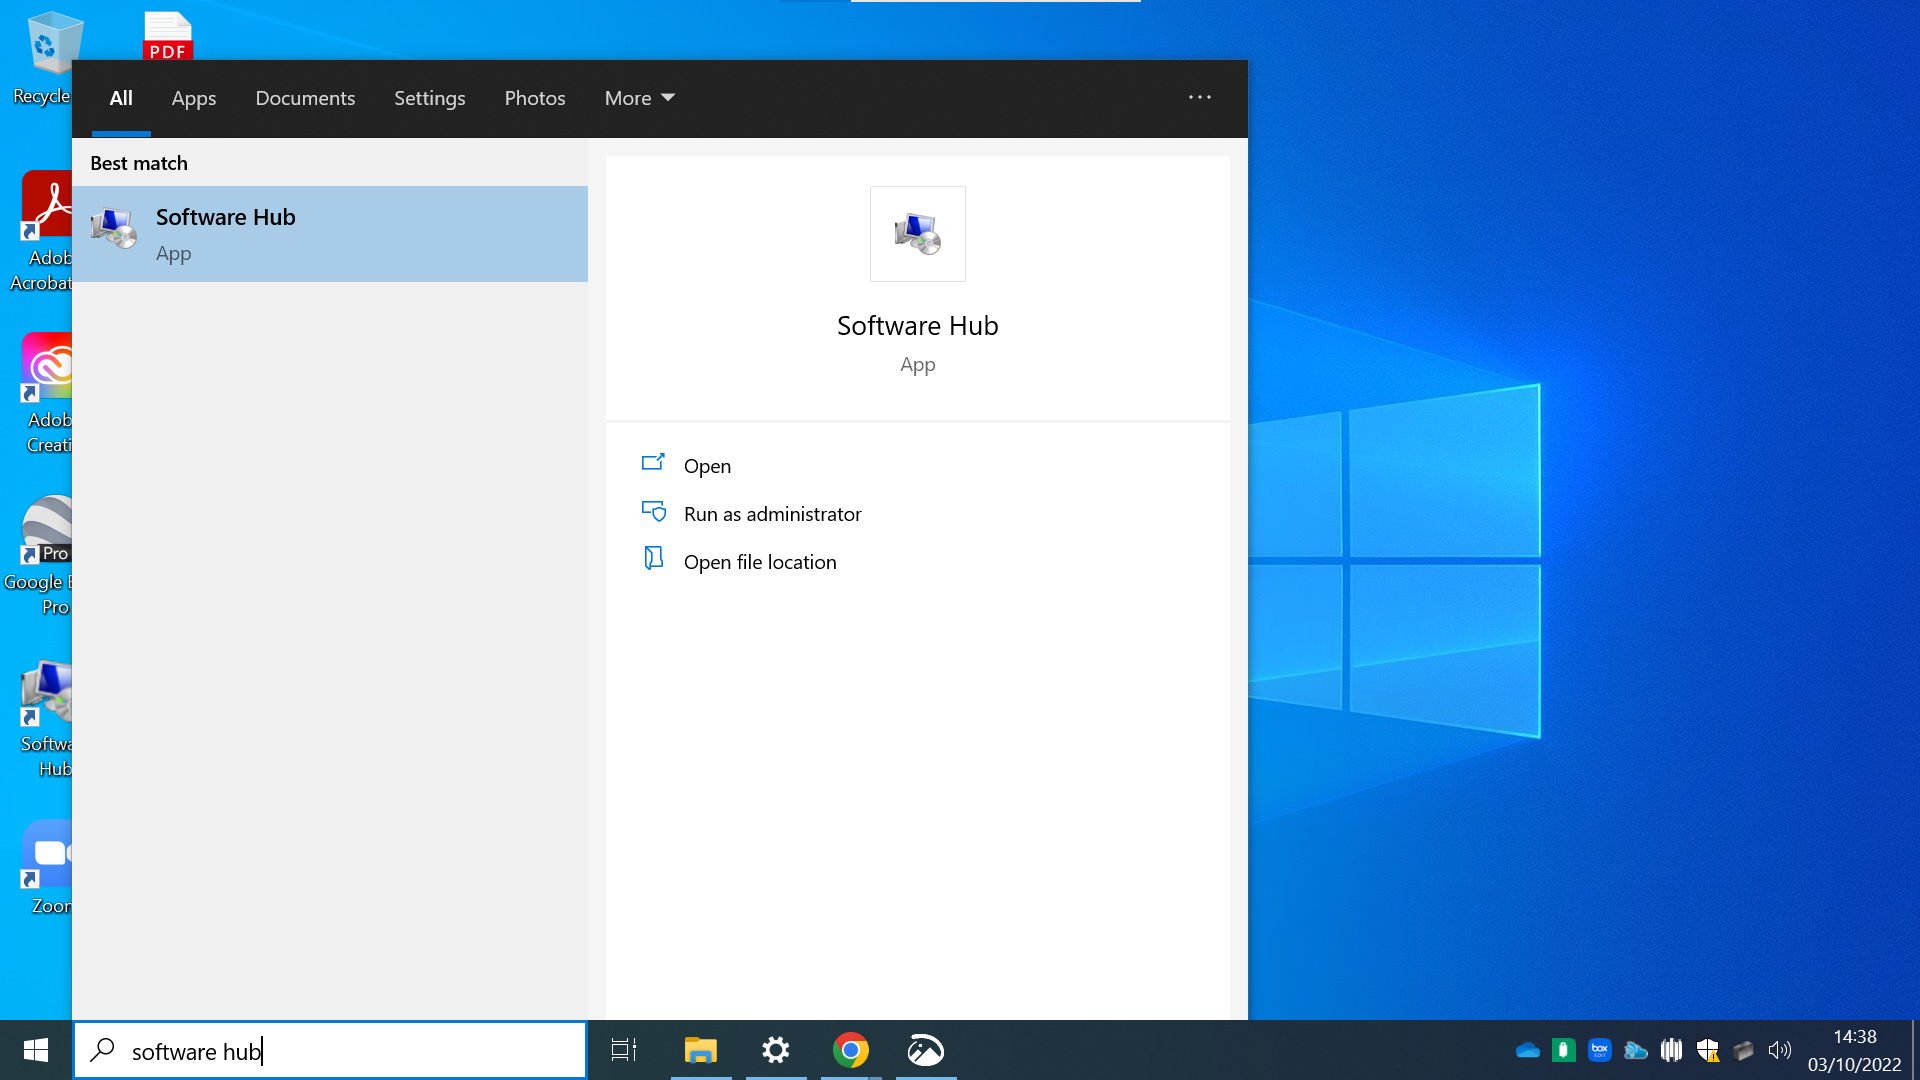
\includegraphics[width=12cm]{Figures/software_hub.png}
\caption{Running Software Hub (first use of Anaconda).}
\label{fig:software_hub}
\end{figure}

Type anaconda into the software hub search box and click Launch
(Fig.~\ref{fig:anaconda_launch}).

\begin{figure}[htbp]  
\centering
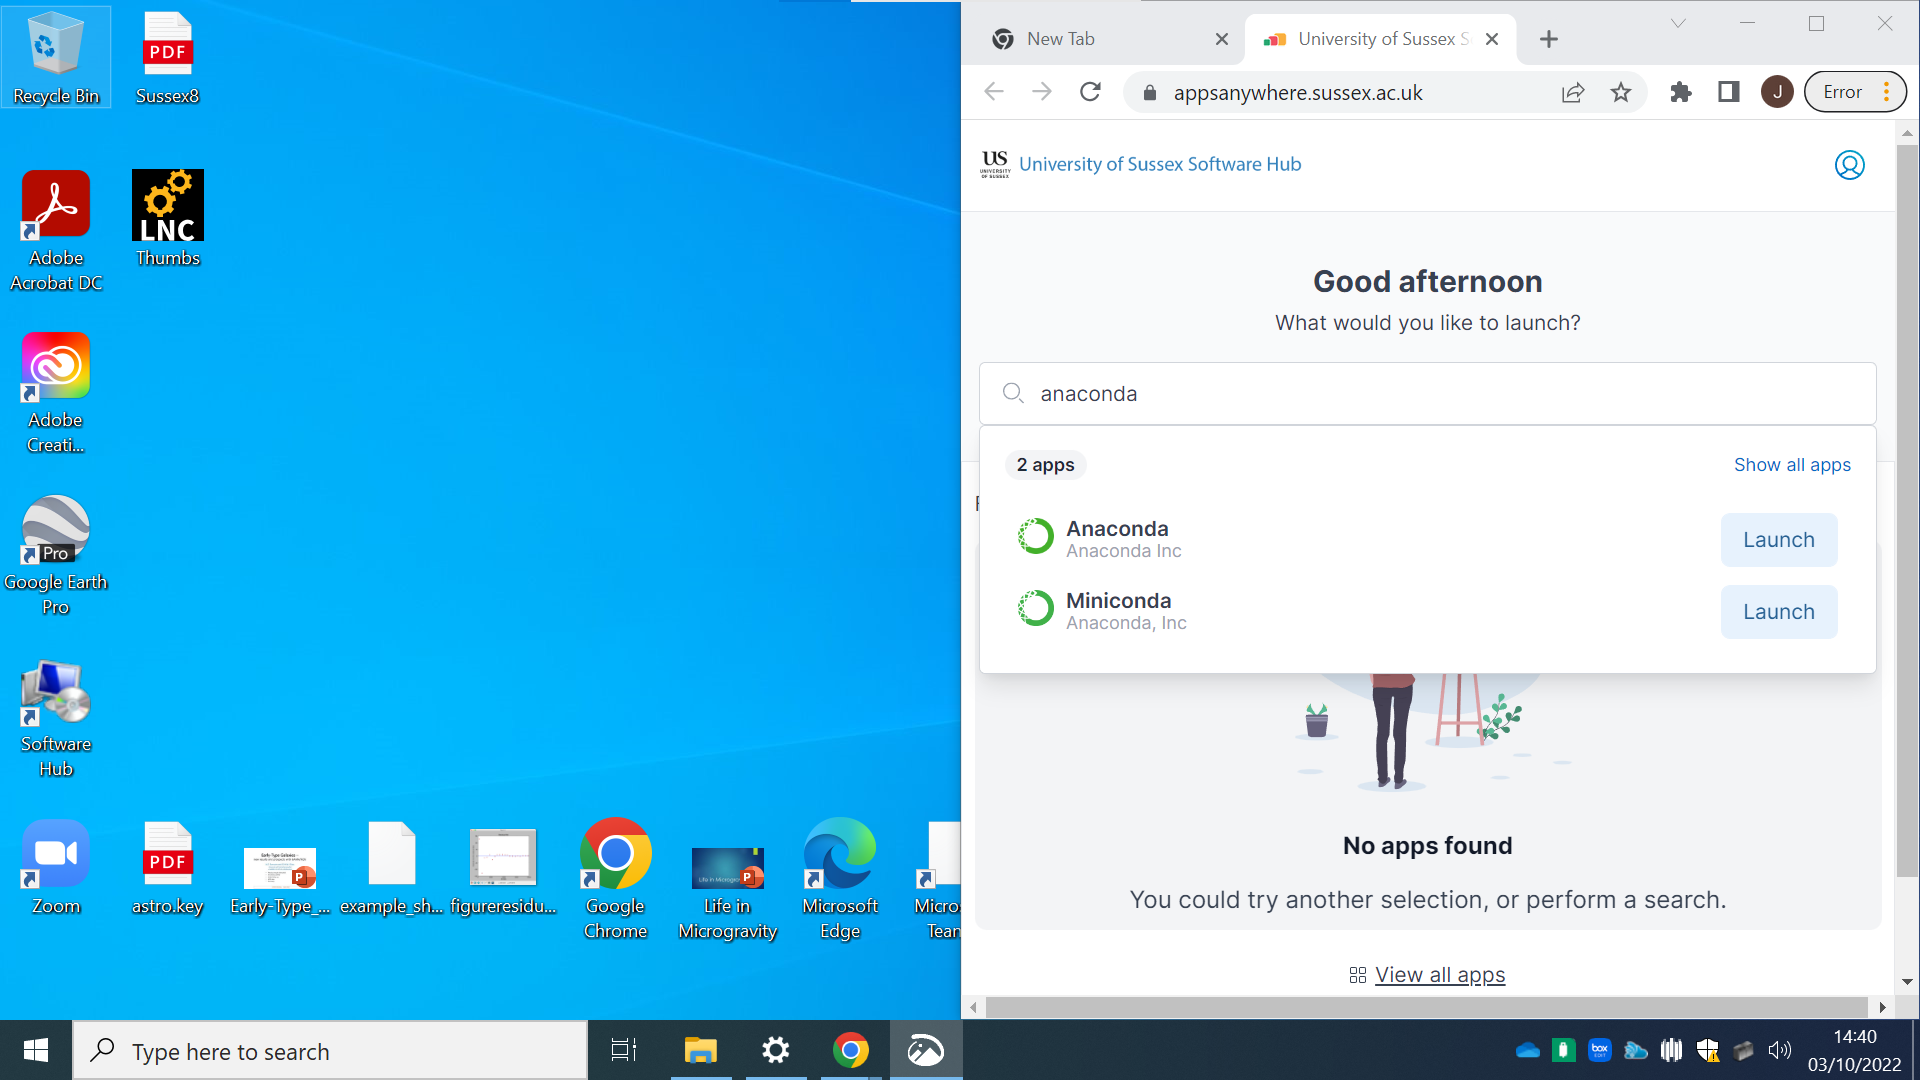
\includegraphics[width=12cm]{Figures/anaconda_launch.png}
\caption{Launching Anaconda (first use).}
\label{fig:anaconda_launch}
\end{figure}

\subsection{Running \texttt{Anaconda} in subsequent sessions}

On subsequent use, you should only need to select Anaconda from the Windows {\tt Start} menu, see Fig.~\ref{fig:programmen}.

\begin{figure}[htbp]  
\centering
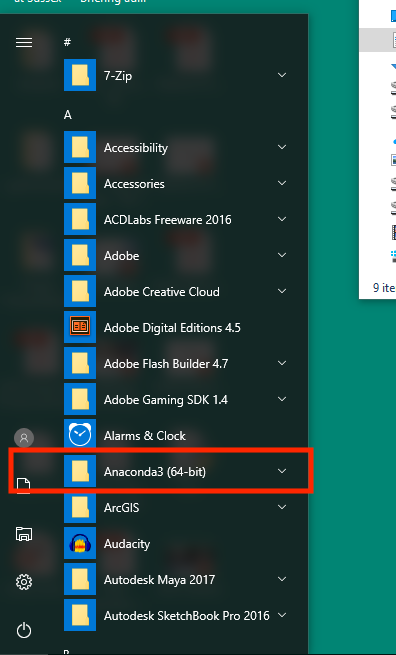
\includegraphics[width=7cm]{Figures/Capture2.PNG}
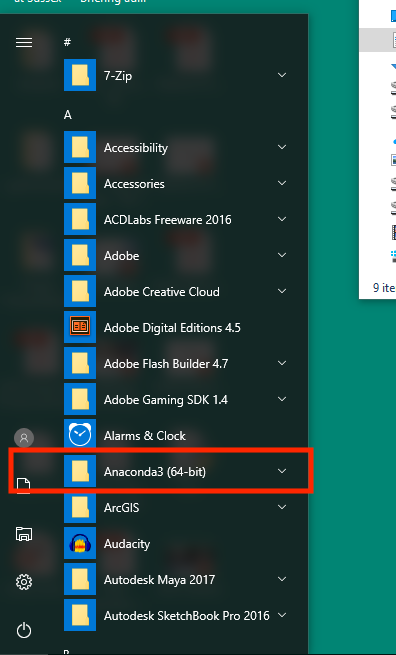
\includegraphics[width=7cm]{Figures/Capture2.PNG}
\caption{Running Anaconda, subsequent use.
  The program menu can be found in the bottom left corner}
\label{fig:programmen}
\end{figure}

\subsection{Running Jupyter Notebook}

After a few moments, the Anaconda Navigator will appear.  From it, launch Jupyter Notebook (Fig.~\ref{fig:jupyter_launch}).

\begin{figure}[htbp]  
\centering
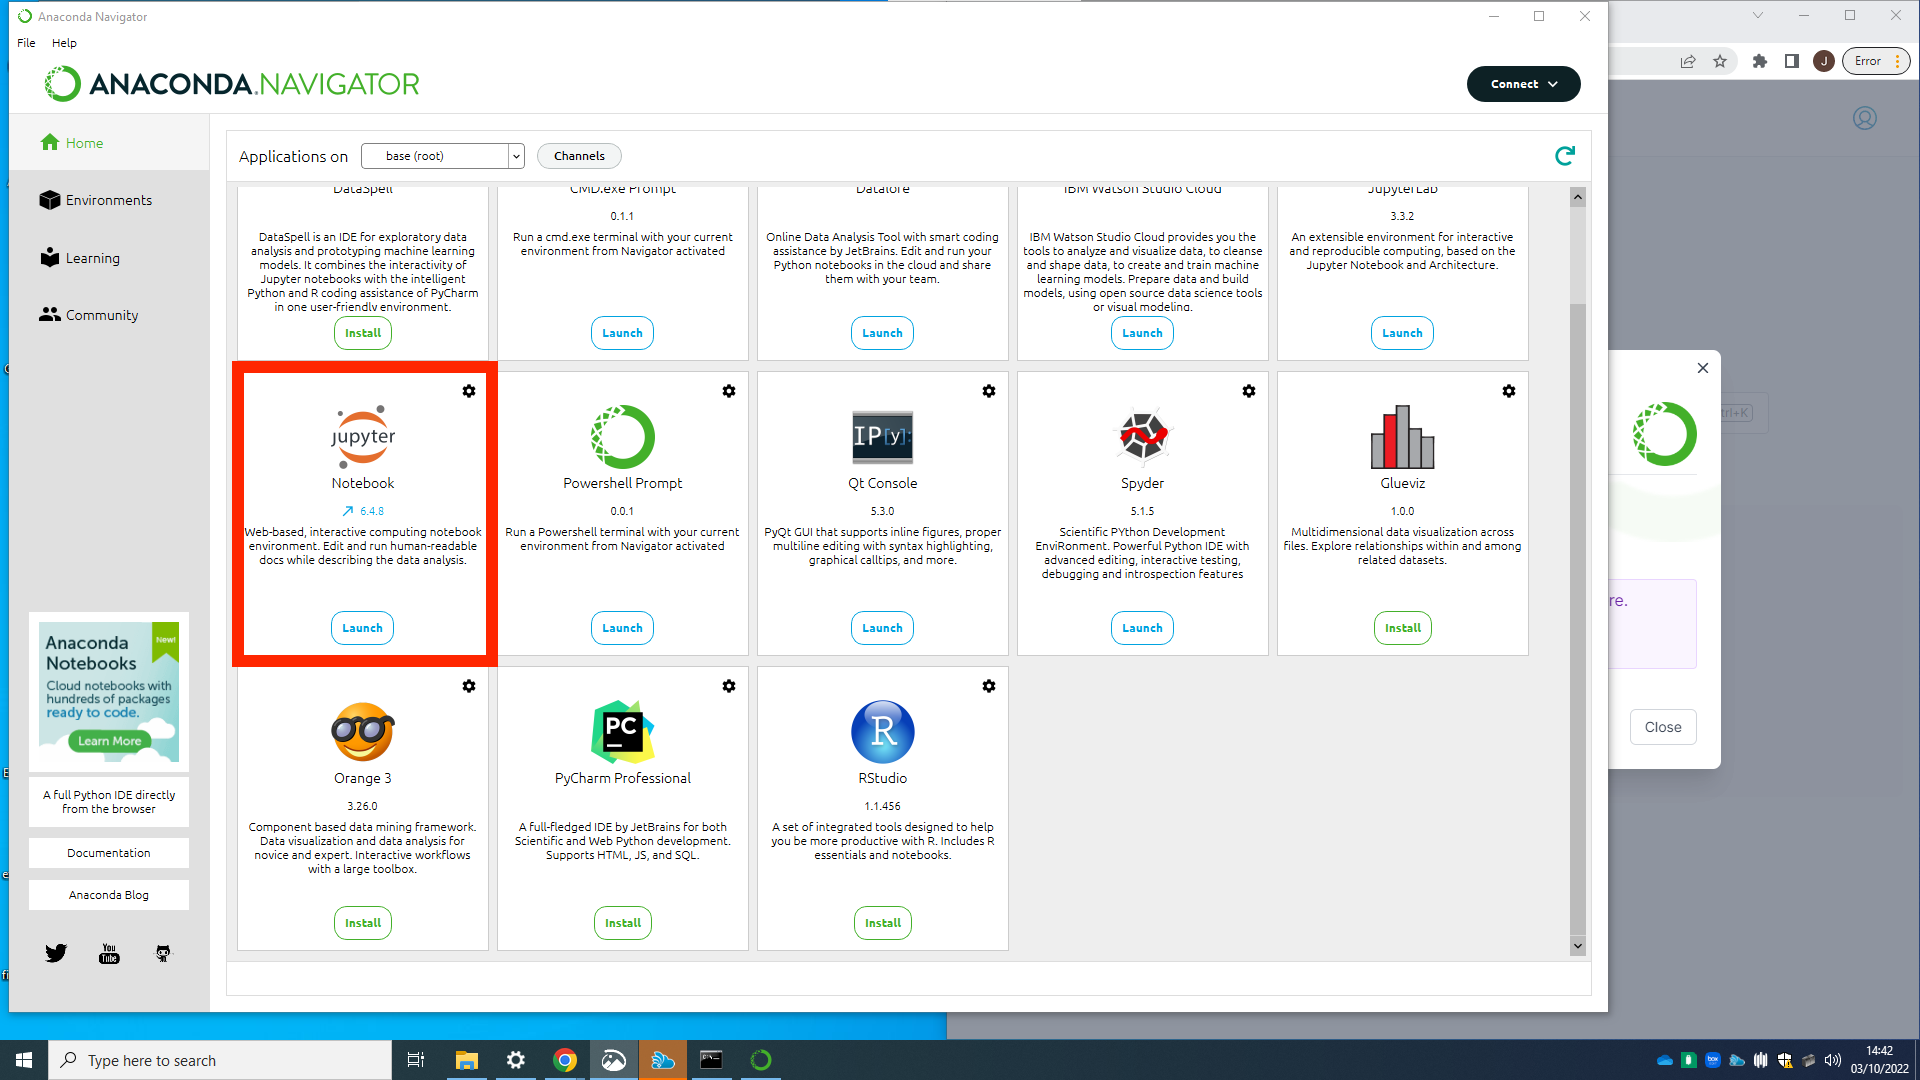
\includegraphics[width=12cm]{Figures/jupyter_launch.png}
\caption{Launching Jupyter.}
\label{fig:jupyter_launch}
\end{figure}

{\bf Important}: any Jupyter notebooks you create should be stored under the folder {\tt OneDrive - University of Sussex}, otherwise they will only be saved on the particular PC that you are using.
Open the {\tt OneDrive - University of Sussex} folder and create a new sub-folder with a name such as \verb|PIP_Python|.
Open that sub-foldder and create a new Jupyter notebook using the {\tt New $\rightarrow$ Python 3} pull-down menu, see Figures~\ref{fig:onedrive} and \ref{fig:python_launch}.

\begin{figure}[htbp]  
\centering
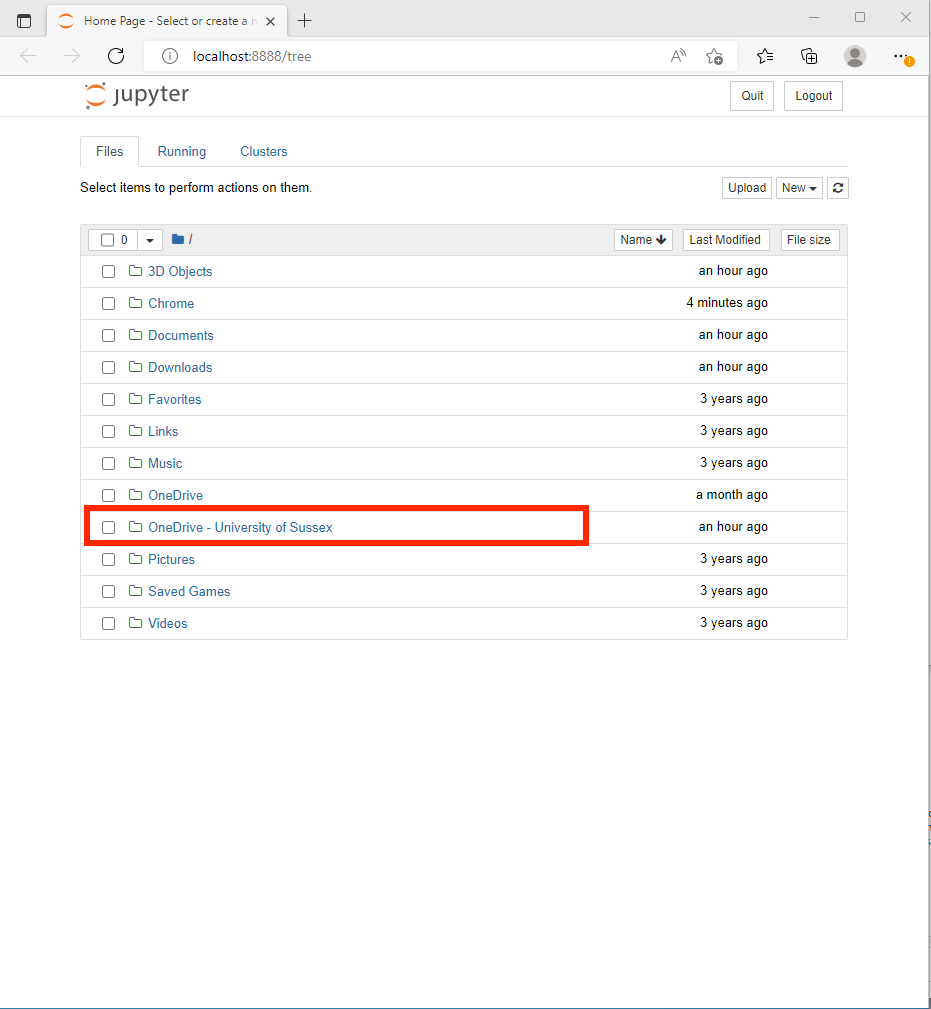
\includegraphics[width=12cm]{Figures/onedrive.png}
\caption{Be sure to save notebooks under {\tt OneDrive - University of Sussex}.}
\label{fig:onedrive}
\end{figure}

\begin{figure}[htbp]  
\centering
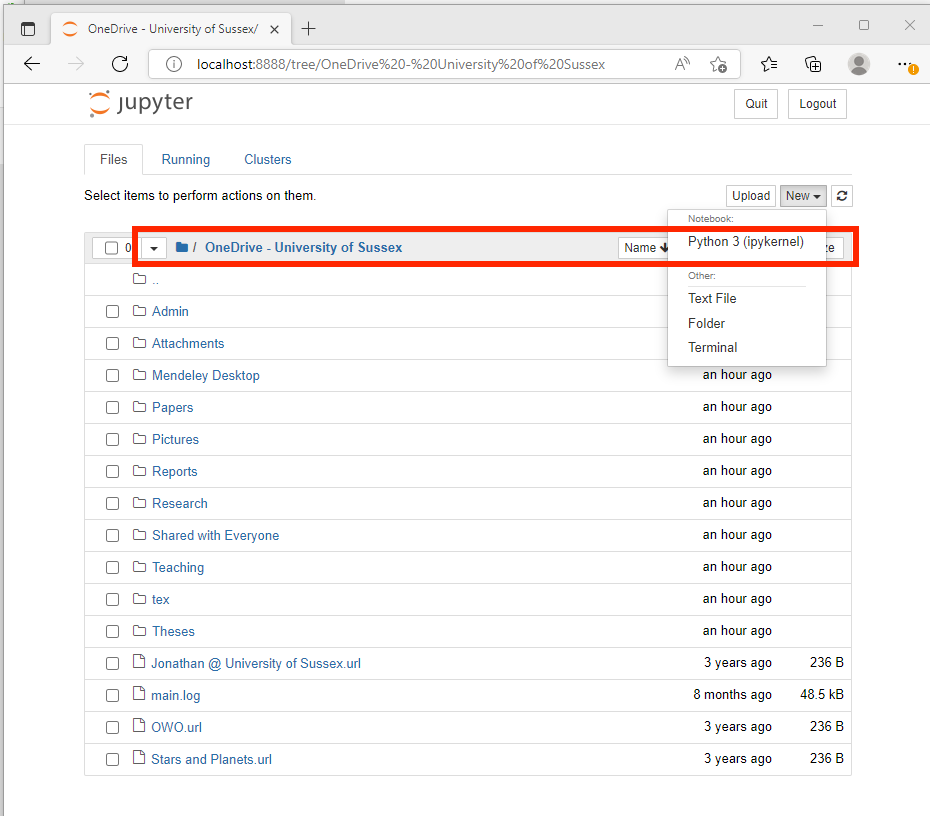
\includegraphics[width=12cm]{Figures/python_launch.png}
\caption{Launching Python.}
\label{fig:python_launch}
\end{figure}

%% On the university machines you can start ``\textbf{jupyter notebook}'' via the Programs
%% Menu (Figure~\ref{programmen}) and the options under Anaconda (Figure~\ref{annaopt}).

%% \begin{figure}[H]  
%% \centering
%% 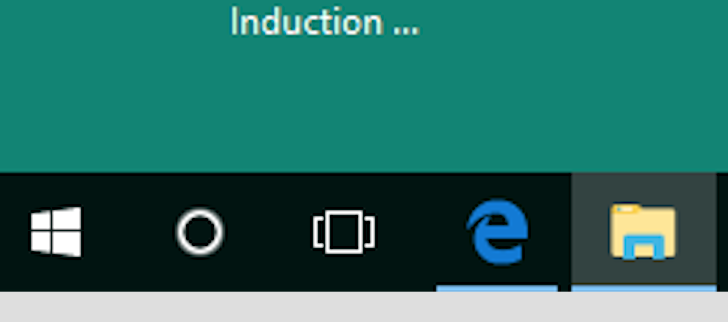
\includegraphics[width=7cm]{Figures/Capture1.PNG}
%% \caption{The program menu can be found in the bottom left corner}
%% \label{programmen}
%% \end{figure}

%% \begin{figure}[H]  
%% \centering
%% 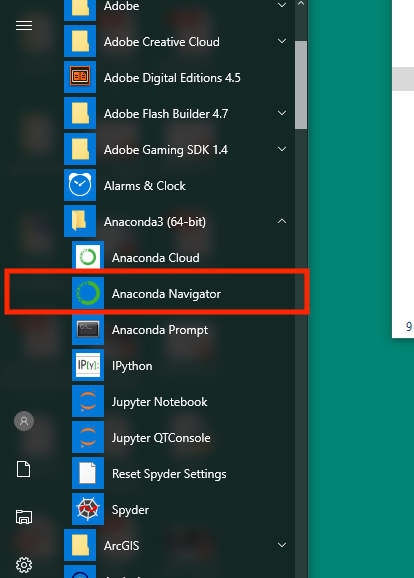
\includegraphics[width=7cm]{Figures/Capture3.PNG}
%% \caption{How to find the \texttt{jupyter} Notebook option via the program menu.}
%% \label{annaopt}
%% \end{figure}

%% The Jupyter Notebook option starts a browser session and a few moments later a \texttt{jupyter} session will appear in your web browser. 
%% Also a console x-term window will pop up immediately (Figure~\ref{xterm}). {\bf Do not close the x-term window as this will stop your \texttt{jupyter} session from working.}  
%% %\end{tcolorbox}

%% %\begin{tcolorbox}[colback=red!5!white,colframe=red!75!black]

%% \begin{figure}[H]  
%% \centering
%% 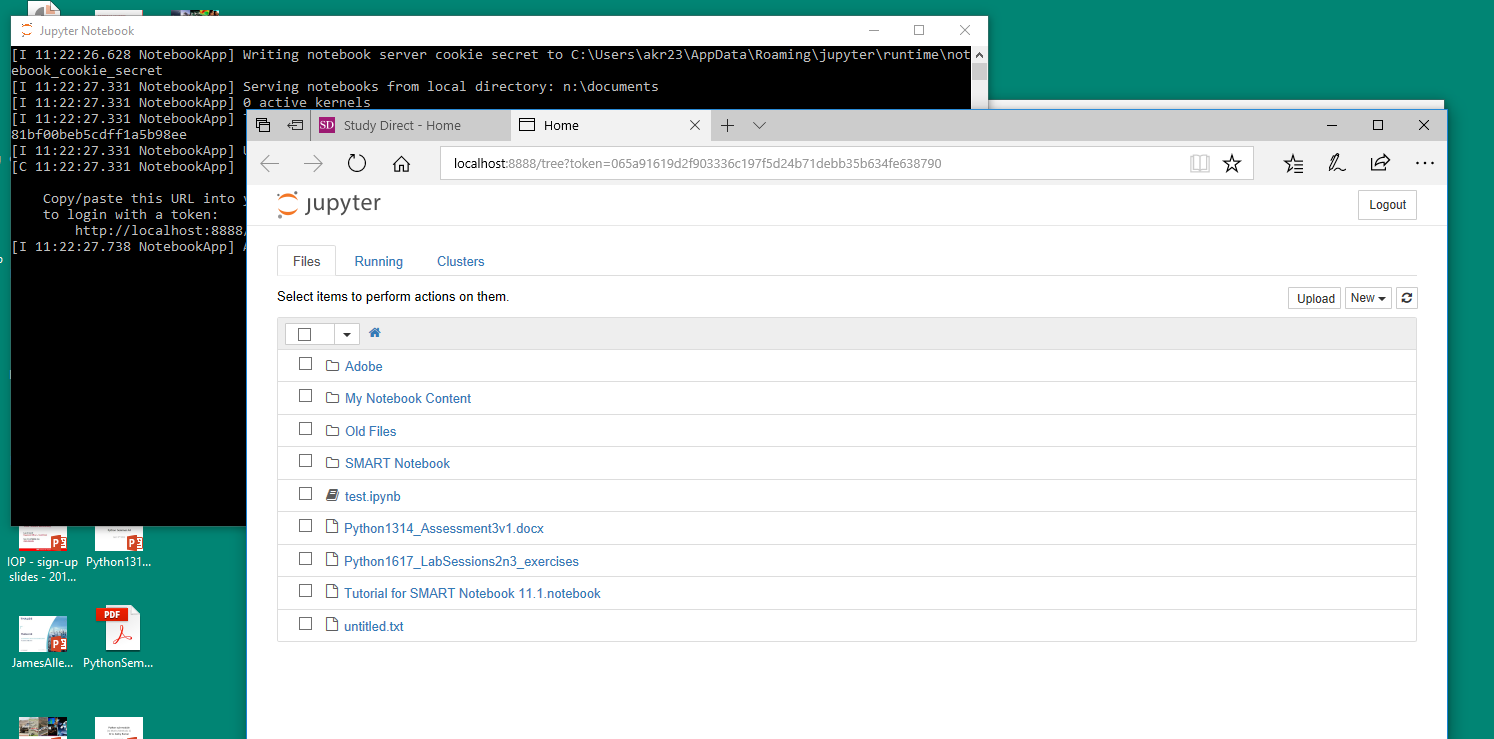
\includegraphics[width=14cm]{Figures/Capture4.PNG}
%% \caption{A \texttt{jupyter} notebook session with the x-term behind it.}
%% \label{xterm}
%% \end{figure}

%% You can now upload to that session an existing \texttt{jupyter} notebook file (extension .ipynb) or you make a new one (see Figure~\ref{OpenNew}).

%% \begin{figure}[H]  
%% \centering
%% 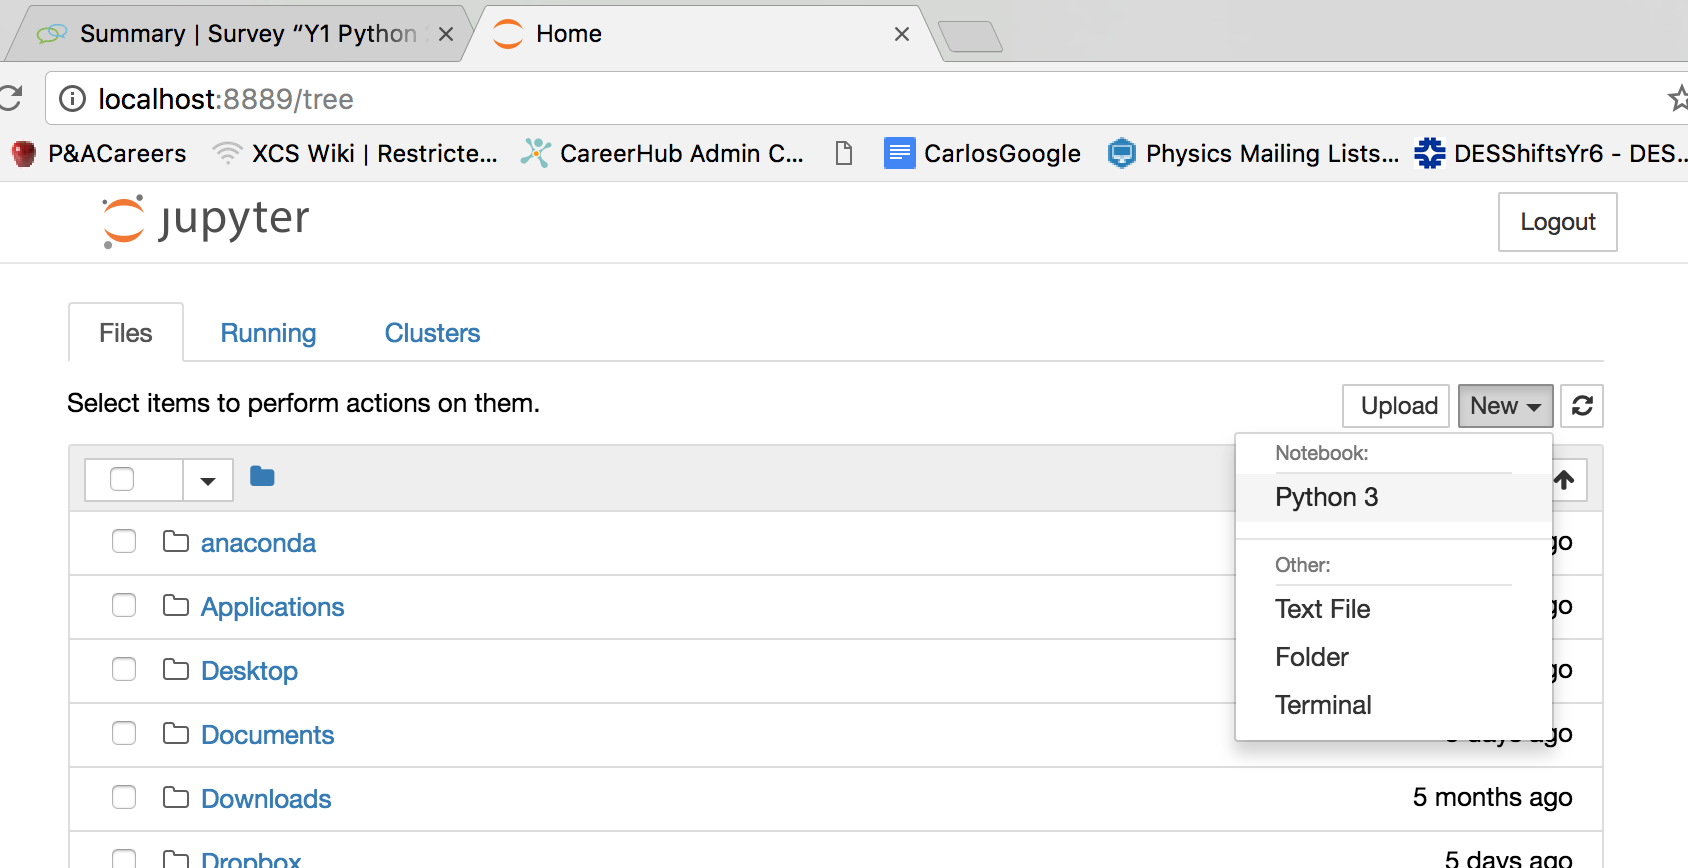
\includegraphics[width=14cm]{Figures/OpenNew.png}
%% \caption{How to open a new \texttt{jupyter} notebook.}
%% \label{OpenNew}
%% \end{figure}

%% %\end{tcolorbox}

\section{Running \texttt{Python} on your own computer}

Throughout this term we will be using \texttt{jupyter notebooks}. \texttt{jupyter} is a web-browser application that allows you to create and share programs, which in our case will be written in \texttt{Python}. This section intends to help you install \texttt{Python} on you personal computer. Should you need to use \texttt{Python} on University computers rather than a personal computer the usual guide for this module can be found in Sec. \ref{StartingPython}. It is worth giving this a read anyway even if you are using a personal computer as it contains some important information.

The easiest way to setup everything you will need for the assessments and labs on your laptop or home PC, is by installing the \href{https://www.anaconda.com}{Anaconda software package} (\url{https://www.anaconda.com}). Anaconda is a `distribution' of \texttt{Python} that has several extra features that make it easier to improve \texttt{Python}'s capabilities; one of the most important is its package manager. 

When you reach chapter \ref{chap:modules}, you'll be introduced to \textbf{modules}, which are pieces of code that other people have written to expand \texttt{Python}'s capabilities. For instance, there are specialist modules for Astrophysics that make it easier for us to do common calculations and operations, such as loading in images from telescopes. \texttt{Python} has a built in way of installing new modules called \texttt{PIP}, but Anaconda adds a more sophisticated package manager which makes sure that all of the modules are the right versions and will work together (amongst other things).

Once you've opened the website, you should:
\begin{enumerate}
    \item Click the download button, at the top right of the website.
    \item Scroll down and select your operating system.
    \item Choose the version you want, \textbf{for this course it should be \texttt{Python} 3.6 or greater}. Should you find yourself using the University system, the version installed there is \texttt{Python} 3.9.
    \item I'd advise the graphical installer for the inexperienced. Windows users must find out what version of Windows is installed, 32 bit or 64 bit. Go to Control Panel - System and Security - System, and you'll find the answer in the system type field.
    \item Now you can download the correct version of Anaconda and install it in the usual way! (Windows users will asked if they wish to add \texttt{Python} to their PATH, and if you want to be able to run \texttt{Python} from command line then you will need to).
    \item When you've installed Anaconda, you'll be able to open Anaconda Navigator.
    \item You'll be presented with several different ways of interacting with \texttt{Python}, if you select Jupyter Notebook (\textbf{not JupyterLab}), then you'll be presented with the interface you use in the lab sessions.
\end{enumerate}

%double check that its version 3.0 - i have a feeling its 3.6?
If you do your assessments on a personal machine \textbf{please ensure that you installed the correct version of \texttt{Python}}. If you fail to check this and your code doesn't work when we try to mark it then I'm afraid its all on you!


\section{``Hello World''}
\label{HelloWorld}

Into your fresh new \texttt{Python-3} \texttt{jupyter notebook}, type {\tt print('hello world')} into the console and then press the ``play'' key. The result should look like Figure~\ref{helloW}. Note that there is a keybord short cut for ``play'': \keys{\ctrl+\enter} ({\tt control+Enter}). For a reference table of useful keyboard shortcuts, look at page \pageref{JupKeyShort}.

\begin{figure}[H]  \centering
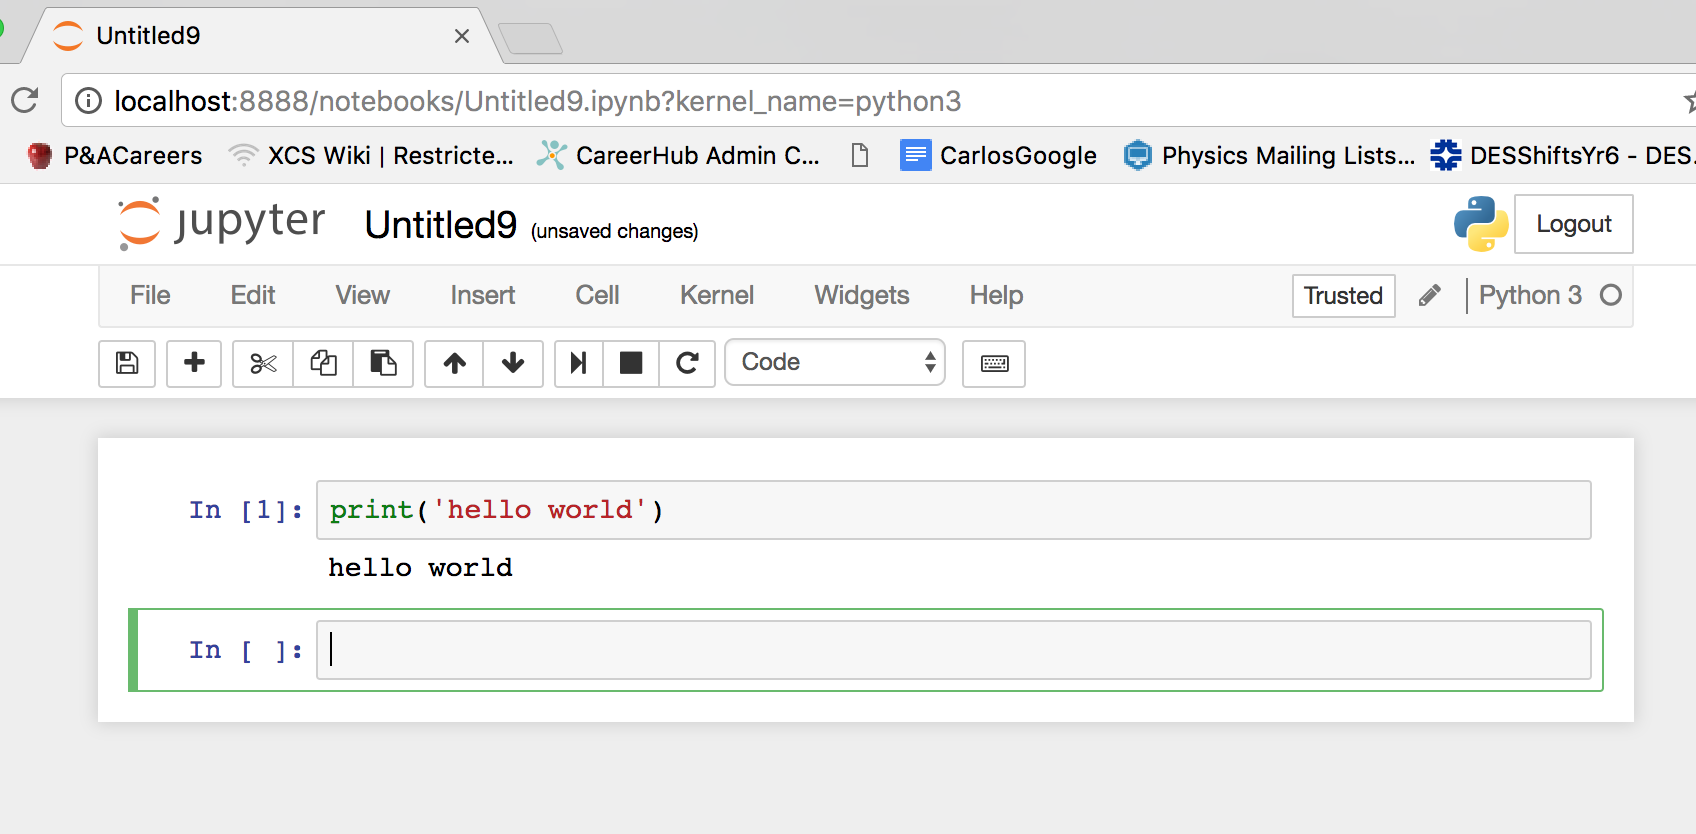
\includegraphics[width=14cm]{Figures/HelloW.png}
\caption{Saying hello to the world using \texttt{jupyter}. Those parentheses and quotation marks are essential: try using {\tt print} without them.}
\label{helloW}
\end{figure}


\subsection{Saving and logging your work}

Make sure to save your work regularly, either by pressing the save button found directly beneath the ``file'' tab, or by pressing \keys{\ctrl+s} ({\tt control+S}). You can then load that file later to start back where you left off. Over the course of the term you will build up a lot of these files, so give them sensible names (e.g. {\tt LabSession1.ipynb} etc.). See Figure~\ref{newname} below.

\begin{figure}[H]  
\centering
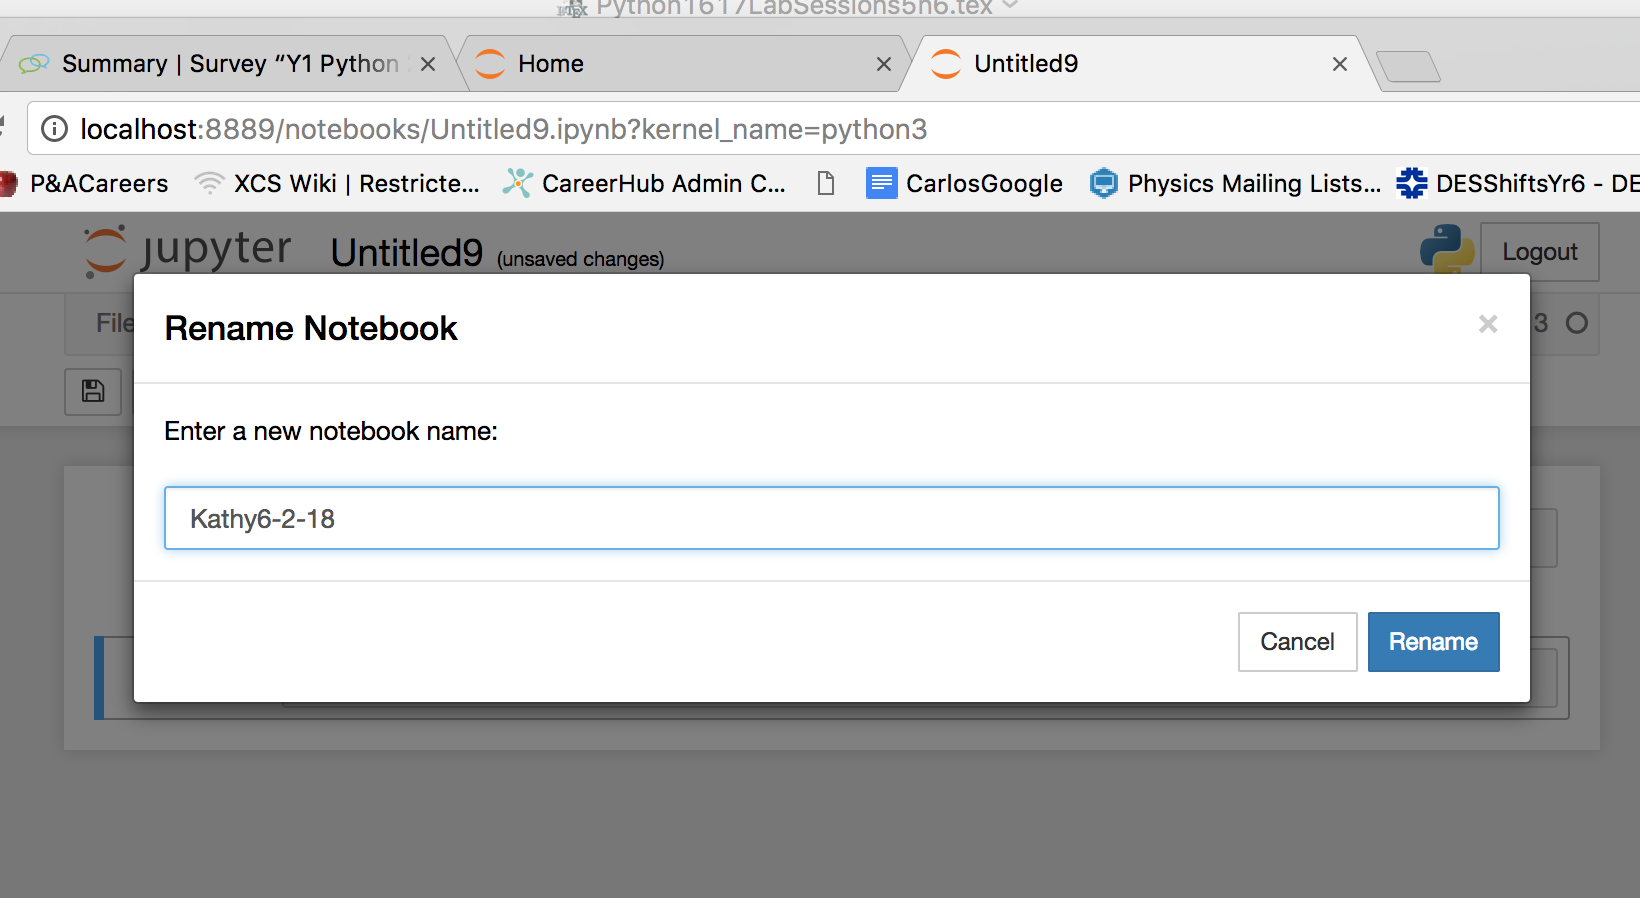
\includegraphics[width=14cm]{Figures/newname.png}
\caption{Your notebook will have a default, not very useful, name, such as ``Untitled9''. It is good practice to rename it to something that will help you remember what is in it. \textbf{Note:} Try to not use spaces in filenames as, although it works on Windows, Linux based systems will not like it - use an underscore instead (a rule to live by).}
\label{newname}
\end{figure}



\subsection{Infinite loops happen... and are very bad}
\label{sec:infiniloop}

If you suspect your code has gone into an infinite loop (a series of instructions that will continue forever), then you need to stop it immediately. Otherwise it may crash your computer (the first year this module was taught, the entire ITS network was disrupted by an infinite loop during a lab session). In \texttt{jupyter}, you go to the ``kernel'' tab and click ``interrupt''. Commit this to memory: infinite loops happen to everyone from time to time.

If you find your screen becomes slow or unresponsive during the infinite loop - you can also double tap "i" on the keyboard when a cell is not selected - this should also interrupt the kernel.


\section{Data types in \texttt{Python}}
\label{dtypes}

In coding, variables are used to store information and give it a descriptive label (the variable name). \texttt{Python} variables can have many different data types, the most common of which are:
\begin{description}
\item[Integer] - These are just integer numbers $(\mathbb{Z})$ such as 1, 53, 8651247 etc.
\item[Floats] - These represent the real numbers $(\mathbb{R})$ to a certain precision. Integers, fractions and irrational numbers can all be stored as floats. E.g, 2.0, 12.5, 6.3215314, $\pi$ etc.
\item[Complex] - These are complex numbers $(\mathbb{C})$, in the form: a+b$i$, 3+5$i$, 7-4$i$ etc. You should have used these in your maths course.\\ Note: In \texttt{Python} the complex number $i$ is represented with $j$, following the engineering convention.
\item[Strings] - These are a sequence of characters. You set the beginning and end of the sequence by enclosing the characters in quotation marks, e.g. `Hello', ``F", `this is also a string'.\\ Note: The quotation marks can be double or single. Choose a convention and stick with it, due to apostrophes it can be best to get in the habit of using ``double quotation marks".
\item[Boolean] - These represent the two values of Boolean logic, True or False.
\item[Lists] - These contain multiple elements and can be different data types. They are also \textbf{mutable} meaning they can be edited after definition. 
\item[Tuples] - Tuples are the same as lists in most respects. However, they are \textbf{immutable} meaning that once created they cannot be changed.
\item[Dictionaries] - This data type contains a set of key:value pairs, with the value being mapped to a \textit{unique} key. Like lists, they are mutable. These are one of the most powerful tools in \texttt{Python} and will be covered in a later practical session.
\end{description}

\noindent During this first lab Session, you'll only need to work with integers, floats and strings. We'll work with the rest later in the term.

\section{Simple calculations with \texttt{Python}}
\label{calculations}
\noindent With integers, floats and complex numbers we can use \texttt{Python} to perform calculations.\\
\noindent Here are some examples. Try them all in your {\tt jupyter} notebook. In the following examples {\tt In}'s and  {\tt Out}'s are included to emulate the {\tt jupyter} output but please note your numbers accompanying them may differ on your screen. 
\noindent Normally we would need to use the print function to see the output (as in section \ref{HelloWorld}), but as you are using {\tt jupyter} and only doing one calculation per cell the result will appear at the bottom.
\vspace*{2ex}

\noindent Adding two integers and complex numbers (add a new cell by clicking the \keys{{+}} button, beneath the ``File'' tab):

\begin{lstlisting}[style=PY]
In [1]: 14 + 3
\end{lstlisting}
\begin{lstlisting}[style=PY, backgroundcolor=\color{white}]
Out[1]: 17
\end{lstlisting}
\begin{lstlisting}[style=PY]
In [2]: 5 + 2j + 4 - 9j
\end{lstlisting}
\begin{lstlisting}[style=PY, backgroundcolor=\color{white}]
Out[2]: (9 - 7j)
\end{lstlisting} 
Subtracting two integers.
\begin{lstlisting}[style=PY]
In [3]: 32 - 8
\end{lstlisting}
\begin{lstlisting}[style=PY, backgroundcolor=\color{white}]
Out[3]: 24
\end{lstlisting}
Multiplying two integers.
\begin{lstlisting}[style=PY]
In [4]: 7 * 9
\end{lstlisting}
\begin{lstlisting}[style=PY, backgroundcolor=\color{white}]
Out[4]: 63
\end{lstlisting}
Computing exponents using $\ast\ast$.
\begin{lstlisting}[style=PY]
In [5]: 2**3
\end{lstlisting}
\begin{lstlisting}[style=PY, backgroundcolor=\color{white}]
Out[5]: 8
\end{lstlisting}
\begin{lstlisting}[style=PY]
In [6]: 25**0.5
\end{lstlisting}
\begin{lstlisting}[style=PY, backgroundcolor=\color{white}]
Out[6]: 5
\end{lstlisting}
You can also combine any of these operations. The rules regarding the order of execution of mathematical operators are the same as you're used to; multiplication and division happen before addition and subtraction etc.
\begin{lstlisting}[style=PY]
In [7]: (4 * (723 + 67)) - 634
\end{lstlisting}
\begin{lstlisting}[style=PY, backgroundcolor=\color{white}]
Out[7]: 2526
\end{lstlisting}
\noindent All of these calculations also work with floats (decimal numbers). \texttt{Python}-3 uses float division (normal division)  by default, therefore when trying out the following calculation we expect the output to be 4.5.
\begin{lstlisting}[style=PY]
In [8]: 27 / 6
\end{lstlisting}
\begin{lstlisting}[style=PY, backgroundcolor=\color{white}]
Out[8]: 4.5
\end{lstlisting}
 The alternative is integer division, where the result of the calculation is rounded down to an integer. This was the default in \texttt{Python}-2, and caused a lot of confusion for new programmers. Even though this no longer applies, it is always best to use floats explicitly, so that you get into good habits.
\begin{lstlisting}[style=PY]
In [9]: 27.0 / 6.0
\end{lstlisting}
\begin{lstlisting}[style=PY, backgroundcolor=\color{white}]
Out[9]: 4.5
\end{lstlisting}
\begin{lstlisting}[style=PY]
In [10]: 27.0 / 6
\end{lstlisting}
\begin{lstlisting}[style=PY, backgroundcolor=\color{white}]
Out[10]: 4.5
\end{lstlisting}
\begin{lstlisting}[style=PY]
In [11]: 27 / 6.0
\end{lstlisting}
\begin{lstlisting}[style=PY, backgroundcolor=\color{white}]
Out[11]: 4.5 
\end{lstlisting}
Python-3 can still perform integer division with the following command 
\begin{lstlisting}[style=PY]
In [12]: 27.0 // 6.0
\end{lstlisting}
\begin{lstlisting}[style=PY, backgroundcolor=\color{white}]
Out[12]: 4.0
\end{lstlisting}
\noindent To perform modulus division (i.e find the remainder) we use the following command.
\begin{lstlisting}[style=PY]
In [13]: 42 % 5
\end{lstlisting}
\begin{lstlisting}[style=PY, backgroundcolor=\color{white}]
Out[13]: 2
\end{lstlisting}
\noindent Here is a table containing the maths commands that come as standard with \texttt{Python}.
\begin{table}[H]
\begin{center}
\caption {Operators calculations}
\begin{tabular}{|l | p{3.5cm}|}
\hline
\texttt{+} & Addition\\\hline
\texttt{-} & Subtraction\\\hline
\texttt{*} & Multiplication\\\hline
\texttt{**} & Exponent\\\hline
\texttt{/} & Division (True)\\\hline
\texttt{//} & Division (Integer)\\\hline
\texttt{\%} & Modulus \\\hline
\end{tabular}
\end{center}
\end{table}

\noindent Now work out the following examples using \texttt{Python}.
\begin{enumerate}
\item 2 + 5
\item 4 - 5
\item 7 $\times$ 8
\item (4 + 7$j$) - (12 - 5$j$)
\item 20$\div$8 (integer division) 
\item 20$\div$8 (float division)
\item 56$\div$9 (integer division) 
\item 6$^{22}$
\item (32 $\times$ 7)$^{2}$
\item (3 + 8$j$) + (1 - 9$j$)
\item $\sqrt{2}$
\item $0^{0}$ (this should be troubling!)
\end{enumerate}

\begin{tcolorbox}[colback=red!5!white,colframe=red!75!black]

In fact, with regards to $0^0$, you might not want this behaviour in your code. In that case, like many other odd behaviours in programming, you are trapped with how the programming language (mis-)behaves. You need to stay aware and code accordingly, and in extreme circumstances use error handling (discussed later). 

\end{tcolorbox}

\section{Using variables for simple maths operations}

We can also assign values to variables, and continue to manipulate them. If you feel a bit hazy about what we mean by a variable, its the $x$ and $y$ in an equation like $y = f(x)$, but in coding it could just as well be $b=f(a)$ or $banana=f(apple)$. Always try and give your variables useful (and slightly amusing) names, so you'll remember what they're for if you come back to a program after a break.\\

\noindent Here we assign 5 to a, 12 to b, -3 to c, and 10.4 to d, and then perform some calculations.
\begin{lstlisting}[style=PY]
In [1]: a = 5
        b = 12
        c = -3
        d = 10.4
        a
\end{lstlisting}
\begin{lstlisting}[style=PY, backgroundcolor=\color{white}]
Out[1]: 5
\end{lstlisting}
\begin{lstlisting}[style=PY]
In [2]: b
\end{lstlisting}
\begin{lstlisting}[style=PY, backgroundcolor=\color{white}]
Out[2]: 12
\end{lstlisting}
\begin{lstlisting}[style=PY]
In [3]: c
\end{lstlisting}
\begin{lstlisting}[style=PY, backgroundcolor=\color{white}]
Out[3]: -3
\end{lstlisting}
\begin{lstlisting}[style=PY]
In [4]: a + b + c
\end{lstlisting}
\begin{lstlisting}[style=PY, backgroundcolor=\color{white}]
Out[4]: 14
\end{lstlisting}
\begin{lstlisting}[style=PY]
In [5]: a - c
\end{lstlisting}
\begin{lstlisting}[style=PY, backgroundcolor=\color{white}]
Out[5]: 8
\end{lstlisting}
\begin{lstlisting}[style=PY]
In [6]: b + 7
\end{lstlisting}
\begin{lstlisting}[style=PY, backgroundcolor=\color{white}]
Out[6]: 19
\end{lstlisting}
We can now perform float and integer division discarding the remainder.
\begin{lstlisting}[style=PY]
In [7]: print(a / 2)
        a // 2
\end{lstlisting}
\begin{lstlisting}[style=PY, backgroundcolor=\color{white}]
        2.5
Out[7]: 2
\end{lstlisting}

\noindent We can also assign the result to a new variable, and use that for further calculations.
\begin{lstlisting}[style=PY]
In [8]: r = a / 2
        r - a // 2
\end{lstlisting}
\begin{lstlisting}[style=PY, backgroundcolor=\color{white}]
Out[8]: 0.5
\end{lstlisting}


\begin{tcolorbox}[colback=red!5!white,colframe=red!75!black]
This style of output is specific to this cell based interface with \texttt{Python} (found in \texttt{jupyter} and another software package called \texttt{iPython}). These will print the contents of \textbf{the last} variable or computation of a cell without the need for a \texttt{print} statement. If you find yourself running a \texttt{Python} script from a .py file or using another Integrated Development Environment (IDE, some are described in section \ref{softwareoptions}) then this will no longer print an output. Other IDEs and \texttt{Python} scripts will also be run as a whole, and not individually cell-by-cell as in \texttt{jupyter}.
\end{tcolorbox}

\subsection{Test your understanding}
Now carry out this task: Define the three variables \texttt{day\_me}, \texttt{month\_me}, \texttt{year\_me} according to your birth date. Then define the three variables \texttt{day\_now}, \texttt{month\_now}, \texttt{year\_now} according to today's date and then figure out how many days you have been alive. This doesn't need to be exact; aim to get within $\pm 200$ days. You can check your answer using one of the many online tools available (use Google to find them).

By now you should have seen that it is more efficient to write several lines of code into a single \texttt{jupyter} cell, and you can use the \keys{\enter} ({\tt Enter}) key to move to a new line. If you need to create a new cell you can either press the \keys{{+}} button under the ``File'' tab or use the keyboard shortcut \keys{\Alt+\enter} ({\tt Alt-Enter}), which will run your current cell before making a new one.

\section{Changing A Variable's Data Type}

You may find yourself in a situation where you need to change the data type of a variable. If we need to convert \texttt{a} to a float we can simply use the \texttt{float} function.
\begin{lstlisting}[style=PY]
In [1]: print(a)
        float(a)
\end{lstlisting}
\begin{lstlisting}[style=PY, backgroundcolor=\color{white}]
        5
Out[1]: 5.0
\end{lstlisting}
Conversely, if we need to convert to an integer we can use the \texttt{int} function.
\begin{lstlisting}[style=PY]
In [2]: int(d)
\end{lstlisting}
\begin{lstlisting}[style=PY, backgroundcolor=\color{white}]
Out[2]: 10
\end{lstlisting}
The value of a variable is not changed by converting it to another data type:
\begin{lstlisting}[style=PY]
In [3]: print(float(a))
        a
\end{lstlisting}
\begin{lstlisting}[style=PY, backgroundcolor=\color{white}]
Out[3]: 5.0
        5
\end{lstlisting}
If we wish to convert \texttt{a} permanently into a float we need to assign it to a new variable, this could be called anything but naming it \texttt{a} overwrites the old value stored in \texttt{a}. We can then proceed with the new variable \texttt{a} containing a float.
\begin{lstlisting}[style=PY]
In [4]: a = float(a)
        print(a / 2)
        a
\end{lstlisting}
\begin{lstlisting}[style=PY, backgroundcolor=\color{white}]
        2.5
Out[4]: 5.0
\end{lstlisting}
It's important to understand that the \texttt{int} function \textbf{does not} round a float up or down, it just truncates it. Lets demonstrate this by defining \texttt{d} so that it would round up to 11.
\begin{lstlisting}[style=PY]
In [5]: d = 10.55
        d
\end{lstlisting}
\begin{lstlisting}[style=PY, backgroundcolor=\color{white}]
Out[5]: 10.55
\end{lstlisting}
\begin{lstlisting}[style=PY]
In [6]: print(int(d))
        d
\end{lstlisting}
\begin{lstlisting}[style=PY, backgroundcolor=\color{white}]
        10
Out[6]: 10.55
\end{lstlisting}
If we wish to actually round a number then we can use the \texttt{round} function.
\begin{lstlisting}[style=PY]
In [7]: e = round(d, 1)
        e
\end{lstlisting}
\begin{lstlisting}[style=PY, backgroundcolor=\color{white}]
Out[7]: 10.6
\end{lstlisting}
The second argument is the number of digits to round to (arguments are values that you pass into a function, here the second argument is 1 and the first is the variable to be rounded). If you didn't give \texttt{round} a second argument, it would round to the nearest whole number and give you the result as an integer.
\begin{lstlisting}[style=PY]
In [8]: round(d)
\end{lstlisting}
\begin{lstlisting}[style=PY, backgroundcolor=\color{white}]
Out[8]: 11
\end{lstlisting}
% To get an integer you can call multiple functions within each other (called nesting), or define new variables to perform each operation on the result of the last operation.
% \begin{lstlisting}[style=PY]
% In [9]: print(int(round(d)))  # nesting functions

%         # Best practice defining new variables
%         rounded_d = round(d)
%         int_d = int(d)
%         print(rounded_d)
%         int_d
% \end{lstlisting}
% \begin{lstlisting}[style=PY, backgroundcolor=\color{white}]
%         11
%         11.0
% Out[9]: 10
% \end{lstlisting}

\section{Commenting}
Comments are added to code to explain the function of lines in a way that a human can understand. They are essential for any project that's more than a few lines long, especially if you're working with other people in a professional setting or you expect to use this code again in the future. Other people may need explanations of code that you think is self-explanatory, and you may not remember how a project works when you come back to it in 6 months.

When writing code just ask yourself this question: Is it immediately clear what a line of code does? (e.g. \texttt{x + 2}, \texttt{print(`Comments are great!!!')}, etc.) If the answer is no, or you're not sure, then put a comment! 

We will be repeatedly telling you to add comments, both during the workshops and the assessments. Comment quality will actually factor into your assessment marks, so get into good habits now. In the last cell of the previous section the different methods for getting an integer were marked with \textbf{comments}. In \texttt{Python}, comments start with a hash (\#)  and are ignored during the execution of the program. Comments can appear anywhere in a line and anything that follows the \# is `commented out', and won't be run as code by \texttt{Python}. 

There are two types, inline comments and block comments. Comments should take the general form:
\begin{lstlisting}[style=PY]
In [1]: # This is a block comment describing the following block of code
        # I am going to do something because... 
        the code that does the something you're doing...
        something particular  # an inline comment about this particular line
\end{lstlisting}

From this point on the examples will have useful comments, though feel free to call us out on any that you think we could do better.

\section{Testing the type of a variable}
\label{variabletype}

Finally, we don't just assign integers and floats to variables, we can also assign strings and any other \texttt{Python} datatype. Also, variable names don't just have to be letters, they can be words too (as long as the word does not match any of \texttt{Python} built in functions like \texttt{print}, or \texttt{int}).

\noindent The fact that variables can be multiple different data types means you may need to find the type of a variable. You can test a variables type very simply using the \texttt{type} function, with this function the output returns of \texttt{str} and \texttt{int} stand for string and integer respectively.
\begin{lstlisting}[style=PY]
In [1]: # Define variables to demonstrate type testing
        f = 45  # integer
        g = 5.2341  # float
        h = 3 + 5j  # complex
        
        type(f)  # test variable f
\end{lstlisting}
\begin{lstlisting}[style=PY, backgroundcolor=\color{white}]
Out[1]: int
\end{lstlisting}
\begin{tcolorbox}[colback=red!5!white,colframe=red!75!black]
When combined with a print statement the \texttt{Python} object itself is printed. This object is an instance of the float class. If this is jibberish don't worry, it is mostly unimportant for the entirety of this module but plenty of resources exist online for learning about \texttt{Python} classes.
\end{tcolorbox}
\begin{lstlisting}[style=PY]
In [2]: print(type(g))  # test variable g and print the result
\end{lstlisting}
\begin{lstlisting}[style=PY, backgroundcolor=\color{white}]
        <class 'float'>
\end{lstlisting}
Note that with a print statement \texttt{jupyter} omits the Out[...], mostly unimportant but don't be confused by it's absence.
\begin{lstlisting}[style=PY]
In [3]: type(h)  # test variable h
\end{lstlisting}
\begin{lstlisting}[style=PY, backgroundcolor=\color{white}]
Out[3]: complex
\end{lstlisting}

\section{A note on the horrors of the insert key}

Every year the same issue comes up, it is very easy to inadvertently press the insert key (\keys{insert}). At first it will appear that nothing has happened, but if you try to type anything within text you've already written, you will start to overwrite the existing characters.

Say you are typing out a print statement,
\begin{lstlisting}[style=PY]
In [1]: print('I want to prit stuff')
\end{lstlisting}
but here you have mistyped and accidentally forgotten the 'n' in print! So you go back to edit, if the insert key is on you would get 
\begin{lstlisting}[style=PY]
In [1]: print('I want to prin stuff')
\end{lstlisting}
as the 'n' has overwritten the 't'. If you encounter this behaviour then insert is the cause, simply press \keys{insert} and problem solved.


\begin{tcolorbox}[colback=red!5!white,colframe=red!75!black]
\section{Integrated Development Environments}
\label{softwareoptions}
A loose definition of an Integrated Development Environment (IDE) might be `a piece of software that provides everything a user needs to write code'. IDEs exist for every programming language, and normally include (at the very least):
\begin{enumerate}
    \item A source code editor - Lets the user write and edit their code.
    \item A debugger - Tools to check for issues with the code.
    \item A compiler - This assembles and runs the code. Different types of programming language approach this differently; languages like C++ have to be compiled (like assembling a machine before you use it) into an `executable' before they're run. \texttt{Python}, on the other hand, is an interpreted language, and is executed line-by-line (like reading a recipe and doing as instructed on each line).
\end{enumerate}

There are a huge number of IDEs to choose from, especially for such a popular language as \texttt{Python}, and ultimately you just have to try a few until you find your favourite. We will summarise a few of the most popular options here, and if you're interested in the subject you can do your own research. Many IDEs are free, but those that do charge often have a student discount option, so look out for that.\\

\begin{itemize}
    \item Text Editors - Although not technically IDEs, text editors like Notepad and Gedit get an honourable mention as you can write code in them and then run it from the terminal. For instance, you could write \texttt{print("hello world")} in a file called test.py, save it, and then run it by typing \texttt{python test.py} in terminal.
    \item Jupyter Notebook - The interface you're familiar with, a relatively lightweight IDE without some of the more complex (and professional level) features you may find in other pieces of software. Its characterised by the cell based approach to coding you will have seen.
    \item Spyder - A more traditional \texttt{Python} IDE than Jupyter, with some more features. If you install Anaconda on your own system, it is included in Anaconda Navigator.
    \item JupyterLab - This is a less lightweight version of Jupyter Notebook, with the same cell based system but more powerful features. Consider it a cross between Jupyter Notebook and Spyder, it is also included in Anaconda Navigator.
    \item PyCharm - This is my personal favourite IDE, and has basically every feature you can ever imagine needing. There is a free version and a paid for professional version (though students can get both for free). It requires a relatively good computer to run it, otherwise it can be a little laggy.
    \item Atom - An infinitely customisable bit of software, whose capabilities can be expanded and adapted by using plug-ins written by other users. 
    \item VS Code is also recommended.
\end{itemize}

\end{tcolorbox}
\hspace{0pt}
\vspace{70mm}
\begin{center}
\Huge{{\bf That's All Folks!}}

\huge{You've completed the first week. See you next time!}
\end{center}
